\chapterimage{head2.png} % Chapter heading image
\chapter{EM Algorithm}
\section{Update the equilibrium probability density}
\begin{definition}
    The basis functions in Def.(\ref{basisfunctions}) were used to update
\begin{align}
    p_{\rm eq}^{k+1}(x) &=\mathbb{E}^k_{X|Y} \left[ \delta(x-X) \right] \\
    &= p^k_{\rm{eq}}(x) \sum_{i,j} \mathbb{E}^k_{X|Y}[a_ib_j] \phi_i(x)\phi_j(x) \\
    &= \sum_{i,j} \psi_i(x) \mathbb{E}^k_{X|Y}[a_ib_j] \psi_j(x).
\end{align}
\end{definition}

\begin{definition}[Update from matrix multiplication]
\begin{align}
    p_{\rm eq}^{k+1}(x) = \mathrm{diag}(\Psi \mathbb{E}^k_{X|Y}[a_ib_j] \Psi^{\dagger})
\end{align}
\end{definition}

\begin{example}[$N_v=3$] In the matrix multiplication, I abbreviate $\mathbb{E}^k_{X|Y}[a_ib_j]$ as $a_ib_j$, and the grids are set like the bottom figure. We will show
\begin{align*}
    p_{\rm eq}^{k+1}(x) &=\sum_{i,j} \psi_i(x) \mathbb{E}^k_{X|Y}[a_ib_j] \psi_j(x) \\
    &= \mathrm{diag}(\Psi \mathbb{E}^k_{X|Y}[a_ib_j] \Psi^{\dagger})
\end{align*}
\begin{center}
    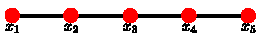
\includegraphics[scale=1.5]{ch2/ex1_grids.pdf}   
\end{center}
\begin{align*} 
&\Psi \mathbb{E}^k_{X|Y}[a_ib_j] \Psi^{\dagger} = \\
&\begin{bmatrix}
    \psi_1(x_1) & \psi_2(x_1) & \psi_3(x_1)  \\
    \psi_1(x_2) & \psi_2(x_2) & \psi_3(x_2) \\
    \psi_1(x_3) & \psi_2(x_3) & \psi_3(x_3)  \\
    \psi_1(x_4) & \psi_2(x_4) & \psi_3(x_4)  \\
    \psi_1(x_5) & \psi_2(x_5) & \psi_3(x_5)  
\end{bmatrix}
\begin{bmatrix}
    a_1 b_1 & a_1 b_2 & a_1 b_3  \\
    a_2 b_1 & a_2 b_2 & a_2 b_3 \\
    a_3 b_1 & a_3 b_2 & a_3 b_3
\end{bmatrix}
\begin{bmatrix}
    \psi_1(x_1) & \psi_1(x_2) & \psi_1(x_3) & \psi_1(x_4) & \psi_1(x_5) \\
    \psi_2(x_1) & \psi_2(x_2) & \psi_2(x_3) & \psi_2(x_4) & \psi_2(x_5) \\
    \psi_3(x_1) & \psi_3(x_2) & \psi_3(x_3) & \psi_3(x_4) & \psi_3(x_5) 
\end{bmatrix} \\
&=\begin{bmatrix}
    \sum_{i=1}^{3}a_i b_1 \psi_i(x_1) & \sum_{i=1}^{3}a_i b_2 \psi_i(x_1) & \sum_{i=1}^{3}a_i b_3 \psi_i(x_1) \\
    \sum_{i=1}^{3}a_i b_1 \psi_i(x_2) & \sum_{i=1}^{3}a_i b_2 \psi_i(x_2) & \sum_{i=1}^{3}a_i b_3 \psi_i(x_2) \\
    \sum_{i=1}^{3}a_i b_1 \psi_i(x_3) & \sum_{i=1}^{3}a_i b_2 \psi_i(x_3) & \sum_{i=1}^{3}a_i b_3 \psi_i(x_3) \\
    \sum_{i=1}^{3}a_i b_1 \psi_i(x_4) & \sum_{i=1}^{3}a_i b_2 \psi_i(x_4) & \sum_{i=1}^{3}a_i b_3 \psi_i(x_4) \\
    \sum_{i=1}^{3}a_i b_1 \psi_i(x_5) & \sum_{i=1}^{3}a_i b_2 \psi_i(x_5) & \sum_{i=1}^{3}a_i b_3 \psi_i(x_5) 
\end{bmatrix}\\
&\begin{bmatrix}
    \psi_1(x_1) & \psi_1(x_2) & \psi_1(x_3) & \psi_1(x_4) & \psi_1(x_5) \\
    \psi_2(x_1) & \psi_2(x_2) & \psi_2(x_3) & \psi_2(x_4) & \psi_2(x_5) \\
    \psi_3(x_1) & \psi_3(x_2) & \psi_3(x_3) & \psi_3(x_4) & \psi_3(x_5) 
\end{bmatrix}\\
&=
\begin{bmatrix}
\sum_{j=1}^{3} b_j \psi_j(x_1) \sum_{i=1}^{3}a_i \psi_i(x_1) &  \sum_{j=1}^{3} b_j \psi_j(x_2) \sum_{i=1}^{3}a_i \psi_i(x_1) &
\cdots & \sum_{j=1}^{3} b_j \psi_j(x_5) \sum_{i=1}^{3}a_i \psi_i(x_1) \\
\sum_{j=1}^{3} b_j \psi_j(x_1) \sum_{i=1}^{3}a_i \psi_i(x_2) &  \sum_{j=1}^{3} b_j \psi_j(x_2) \sum_{i=1}^{3}a_i \psi_i(x_2) &
\cdots & \sum_{j=1}^{3} b_j \psi_j(x_5) \sum_{i=1}^{3}a_i \psi_i(x_2) \\
\sum_{j=1}^{3} b_j \psi_j(x_1) \sum_{i=1}^{3}a_i \psi_i(x_3) &  \sum_{j=1}^{3} b_j \psi_j(x_2) \sum_{i=1}^{3}a_i \psi_i(x_3) &
\cdots & \sum_{j=1}^{3} b_j \psi_j(x_5) \sum_{i=1}^{3}a_i \psi_i(x_3) \\
\sum_{j=1}^{3} b_j \psi_j(x_1) \sum_{i=1}^{3}a_i \psi_i(x_4) &  \sum_{j=1}^{3} b_j \psi_j(x_2) \sum_{i=1}^{3}a_i \psi_i(x_4) &
\cdots & \sum_{j=1}^{3} b_j \psi_j(x_5) \sum_{i=1}^{3}a_i \psi_i(x_4) \\
\sum_{j=1}^{3} b_j \psi_j(x_1) \sum_{i=1}^{3}a_i \psi_i(x_5) &  \sum_{j=1}^{3} b_j \psi_j(x_2) \sum_{i=1}^{3}a_i \psi_i(x_5) &
\cdots & \sum_{j=1}^{3} b_j \psi_j(x_5) \sum_{i=1}^{3}a_i \psi_i(x_5)
\end{bmatrix}
\end{align*}

\end{example}